%-------------------------------------------------------------------------------
% Este arquivo contém a sua funtamentação teórica
%-------------------------------------------------------------------------------
\chapter{Fundamentação Teórica}

A necessidade de apoiar o desenvolvimento da EAD tem feito surgir novas teorias,
métodos, abordagens de ensino e tratamento das informações, geradas nas diversas
tecnologias usadas na EAD. Serão abordadas nas seções seguintes, as principais
temáticas que serão usadas neste estudo, dando-lhe as bases teóricas necessárias
para o seu desenvolvimento e compreensão dos seus resultados futuros.

\section{Teoria da Distância Transacional}

Em 1972, Michael Grahame Moore propôs teorias pioneiras para a educação a
distância. Essa teoria seria posteriormente denominada de Teoria da Distância
Transacional (TDT). Ao longo de mais de 40 anos desde de seus fundamentos
iniciais, o próprio autor e outros pesquisadores trataram de atualizá-la,
principalmente em razão da evolução tecnológica e da necessidade de sua
renovação periódica. Os textos originais do autor estão nas suas obras de 1973,
1993 e 2013 \cite{moore1973transational}.

Em seus estudos, \citeonline{moore2008teoria} afirmou que, na EAD
não existe apenas uma distância física entre professores e alunos mas também uma
distância psicológica. Esta é uma teoria que descreve as relações
estudante-professor e intra-estudante e suas consequências na qualidade do
ensino a distância. Na TDT, este universo de relações pode ser estudado
baseando-se na construção dos componentes ou construtos elementares deste campo,
sendo eles, a estrutura dos programas e cursos, a interação entre alunos e
professores ou diálogo e a próprio grau de autonomia e independência do
estudante. Uma teoria educacional que afirma que a educação a distância tem a
sua própria identidade e características pedagógicas distintivas. É a primeira,
se não a única, teoria em EAD que pode ser utilizada para testar hipóteses. Como
outras teorias, pode ser usada para calcular uma heurística, utilizada para
tomada de decisões em projetos de cursos da EAD \cite{moore2008teoria}.

\citeonline{dewey1960knowing} elaboraram o conceito de transação, que, conforme
foi exposto posteriormente por \citeonline{boyd1980redefining}, denota a
interação entre o ambiente, os indivíduos e os padrões de comportamento numa
dada situação. Uma transação, em educação a distância, é a interação entre
professores e alunos que estão espacialmente separados. Como foi definido por
\citeonline{moore2008teoria}, essa separação cria padrões especiais de
comportamento que afetam tanto o ensino quanto o aprendizado. Derivado da
separação, surge um espaço psicológico e comunicacional propício a
mal-entendidos nas intervenções instrutor-aluno. A esta separação é dado o nome
de Distância Transacional (DT).

Distância Transacional é o espaço psicológico e comunicacional gerado pela
separação entre alunos e professores em um ambiente de educação a distância. O
termo distância se refere a este espaço psicológico e não a distância física
entre os participantes de um curso EAD \cite{goel2012transactional}. Esta
distância é uma função de três construtos: diálogo, estrutura do curso e
autonomia do aluno.

Faz-se necessário lembrar que, segundo \citeonline{moore2008teoria} a
distância transacional não é um valor fixo ou dicotômico, na verdade é um valor
relativo e contínuo. E é diferente para cada estudante, mesmo entre os que
compartilham o mesmo curso. Foi apontado por \citeonline{rumble1986planning} que
existe uma DT mesmo em cursos presenciais. A vista desses argumentos, podemos
dizer que a EAD é um subconjunto da educação e os estudos realizados em EAD
podem auxiliar a teoria e prática da educação tradicional. Porém, em uma
situação classificada como EAD, a distância entre os participantes - professores
e alunos - é grande o suficiente para justificar a investigação de técnicas
próprias de ensino-aprendizagem.

Os procedimentos de ensino se dividem em dois grupos, e acontece também um
terceiro grupo de variáveis que descreve o comportamento dos alunos. A DT é uma
função desses três grupos de variáveis. Essas variáveis não são tecnológicas ou
comunicacionais, na verdade, são variáveis em ensino e aprendizagem e na
interação entre ensino e aprendizagem. Em TDT, estes grupos de variáveis recebem
o nome de Diálogo, Estrutura e Autonomia do Aluno \cite{moore2008teoria}.

\subsection{Diálogo}

Diálogo foi originalmente definido por \citeonline{moore1973transational} como
sendo interações focadas, positivas, propositais entre o professor e os alunos.
Ainda segundo Moore, o diálogo ocorre entre professores e alunos quando alguém
ensina e os demais reagem. Interações negativas ou neutras não são classificadas
como diálogo. O diálogo deve ser direcionado para o aperfeiçoamento da
compreensão por parte do aluno.

``A extensão e natureza do diálogo são determinadas pela filosofia educacional
da instituição responsável pelo projeto do curso, pelas personalidades do
professor e do aluno, pelo tema do curso e por fatores ambientais.''
\cite[p.~438]{cabau2018teoria}.

\citeonline{moore2008teoria} cita meios de comunicação como um importante
fator ambiental na EAD, no entanto, relata ser importante que outras variáveis
sejam atendidas à medida que a EAD amadurece, as variáveis destacadas por Moore
foram: projeto de curso, seleção e treinamento de instrutores e o estilo de
aprendizagem dos alunos.

É o mediador central da DT e referenciado como medida de aprendizado ao passo
que a DT seria uma medida de não-aprendizado. No entanto, já que o diálogo não
se limita apenas à interação professor-aluno, especialmente com os avanços da
EAD provendo novas formas de interações entre estudantes, diversos pesquisadores
vêm propondo a inclusão de interações/relacionamentos entre alunos no conceito
de diálogo
\cite{benson2009addressing,chen1999dimensions,huang2016understanding}.

\subsection{Estrutura do curso}

A estrutura do curso diz respeito aos elementos do projeto, bem como, divisão do
curso em unidades, objetivos, estratégias institucionais e métodos de avaliação.
A estrutura transmite a flexibilidade ou rigidez dos elementos do curso. É também
responsável pela facilitação ou não-facilitação do diálogo
\cite{moore2008teoria}.

Bem como o diálogo, a estrutura do curso é uma variável qualitativa, e a
medida da estrutura em um programa EAD é, normalmente, determinada pela natureza
dos meios de comunicação empregados, e também pela filosofia e personalidade dos
professores, pelas personalidades dos alunos e pelas restrições impostas pelas
instituições educacionais \cite{moore2008teoria}.

Embora Moore atribua como qualitativa o tipo de variável relacionada ao diálogo
e à estrutura, diversos estudos recentes mostraram que é possível quantificar e
mensurar esses componentes da TDT
\cite{zhang2003transactional,horzum2011developing,paul2015revisiting,
ramos2016abordagem}.

\citeonline{ramos2016mapeamento}, propôs o mapeamento do comportamento de
usuários de um \textit{Learning Management System} (LMS), em variáveis que
representam os contrutos da TDT. O objetivo foi descrever e validar um conjunto
de variáveis com as quais esses construtos podem ser medidos, permitindo o
desenvolvimento de pesquisas na área, assim como a obtenção destas medidas a
qualquer momento do curso e sem a necessidade de questionários. A criação e
validação de um conjunto final de variáveis foi feita a partir da Análise
Fatorial Confirmatória (CFA), que apontou como cada construto pode ser
representado por um conjunto de atributos obtidos a partir do banco de dados do
LMS.

Em cursos gravados em fitas, discos, ou mesmo cursos televisionados a estrutura
é rígida e o diálogo não existe, pois não é possível reorganizar o conteúdo para
levar em consideração as interações de um aluno. Em contrapartida cursos por
teleconferências, permitem ampla variedade de respostas alternativas do
instrutor às perguntas dos participantes. Um curso altamente estruturado não
possibilita o diálogo professor-aluno, consequentemente a DT entre alunos e
professores aumenta. No entanto, o contrário não pode ser generalizado. ``\ldots
a extensão do diálogo e a flexibilidade da estrutura variam de programa para
programa. É esta variação que dá a um programa maior ou menor distância
transacional que outro'' \cite{moore2008teoria}.

Em um programa com pequena DT os alunos recebem instruções e orientações por
meio do diálogo com o instrutor, neste caso é possível ter uma estrutura aberta,
que dê respaldo para tais interações. Em programas com maior DT é necessário uma
estrutura robusta, materiais didáticos que forneçam todas as orientações,
instruções e aconselhamentos que o instrutor puder prever, mas sem a
possibilidade de alterações por meio de diálogo aluno-professor
\cite{moore2008teoria}.

Temos então que, em programas mais distantes, os alunos precisam se
responsabilizar em escolher quais atividades e avaliações serão feitas e quando
serão feitas. Mesmo que o curso seja bem estruturado, o estudante, na falta de
diálogo, decidirá quais atividades serão realizadas, quando, e qual a
importância de cada uma. Sendo assim, quanto maior a DT mais é exigido uma
autonomia do aluno \cite{moore2008teoria}.


\subsection{Autonomia do aluno}

No período do surgimento da TDT, década de 1970, ela representava a fusão de
duas tradições pedagógicas presentes nos anos 1960 que pareciam contraditórias.
Uma, a tradição humanística, que valorizava o diálogo aberto, não-estruturado e
interpessoal, tanto na educação quanto no aconselhamento. A outra, a tradição
behaviorista que valorizava o projeto sistemático da instrução, baseado em
objetivos comportamentais com o máximo de controle do processo de aprendizagem
por parte do professor. No início dos anos 1970, a EAD era dominada pela
tradição behaviorista. Tanto que, o título do primeiro trabalho sobre a TDT de
\citeonline{moore1972learner} foi: ``A autonomia do aluno --- a segunda dimensão
da aprendizagem independente''. Neste trabalho Moore afirmou que: ``educadores
por correspondência universitários limitavam o potencial do seu método ao
negligenciar a habilidade dos alunos em compartilharem a responsabilidade por
seus próprios processos de aprendizagem'' \cite{moore2008teoria}.

O termo ``autonomia do aluno'' foi escolhido para descrever os padrões de
comportamento de alunos que usavam materiais didáticos e programas de ensino
para atingir seus próprios objetivos, à sua maneira e sob seu próprio controle
\cite{moore2008teoria}.

\apudonline{boyd1966psychological}{moore2008teoria} criou uma descrição para o
comportamento ideal de uma pessoa emocionalmente independente de um instrutor,
uma pessoa que pode abordar assuntos diretamente sem ter um adulto participando
de um conjunto de papéis de mediação entre o aluno e a matéria de estudo.

Autonomia do aluno  se refere a capacidade de se auto-direcionar.
\citeonline{moore2008teoria} definiu o estudante autônomo ideal como ``a
pessoa emocionalmente independente de um professor'' e quem ``tem capacidade de
abordar o assunto estudado diretamente sem a ajuda de um instrutor''. Diferente
da estrutura do curso e do diálogo, é um fator que depende apenas do aluno. Um
aprendiz pouco autônomo pode precisar de um direcionamento maior e uma estrutura
mais rígida \cite{huang2016understanding}.

\section{Evasão de alunos na EAD}

O censo mais recente, no período da escrita deste trabalho, realizado pela
Associação Brasileira de Educação a Distância (ABED), com dados de 2016,
consultou 340 instituições em todo o país, formadoras e fornecedoras de de
produtos e serviços para EAD \cite{abed2016ead}.

De acordo com o Censo EAD.BR 2016 as taxas de evasão informadas pelos
respondentes recaíram principalmente entre 11\% e 25\%. O censo também revelou
que entre os respondentes, as taxas de evasão dos cursos semipresenciais tem
taxa de evasão menor que cursos totalmente a distância. A Tabela
\ref{tableEvasionTax1} compara os índices dos 4 últimos censos realizados pela
ABED
\cite{abed2013ead,abed2014ead,abed2015ead,abed2016ead}

\begin{table}[!htb]
  \centering
  \caption{\label{tableEvasionTax1} Taxas de evasão ao longo dos anos segundo o censo realizado pela ABED}
  \begin{tabular}{@{}lllll@{}}
    \toprule
    \multicolumn{1}{c}{\multirow{2}{*}{\textbf{\begin{tabular}[c]{@{}c@{}}Taxas de evasão \\ declaradas\end{tabular}}}} & \multicolumn{4}{c}{\textbf{\begin{tabular}[c]{@{}c@{}}Percentuais de instituições\\ declarantes, por faixa\end{tabular}}} \\ \cmidrule(l){2-5}
    \multicolumn{1}{c}{} & \textbf{2013} & \textbf{2014} & \textbf{2015} & \textbf{2016} \\ \midrule
    Até 25\% & 65\% & 50\% & 53\% & 58\% \\
    Entre 26 e 50\% & 24\% & 38\% & 40\% & 19\% \\
    Acima de 50\% & 2\% & 2\% & 7\% & 1\% \\
    Não declararam & 9\% & 10\% & - & 22\% \\ \bottomrule
  \end{tabular}
  \Otherguydidthis{abed2013ead,abed2014ead,abed2015ead,abed2016ead}
\end{table}

Entre os motivos para evasão investigados e declarados no censo, questões
financeiras e falta de tempo foram os citados como os que geram maior evasão.
Houve uma parcela considerável de respondentes que acredita que a evasão não é
um problema em cursos totalmente a distância pois os participantes podem sempre
retornar.

Em cursos livres o motivo mais citado foi a falta de tempo, e também grande
parte dos respondentes acredita que os alunos de cursos livres não corporativos
sempre podem retornar.

O Censo EAD.BR 2016 apontou que cursos presenciais, semipresenciais e
corporativos possuem mecanismos que vão além do conteúdo e da interação online
com professores para manter seus alunos engajados. Já os cursos totalmente a
distância e cursos livres não corporativos dependem apenas da experiência do
aluno com o conteúdo e com seus professores e tutores.

A Tabela \ref{tableEvasionTax2} apresenta dados dos indicadores da evasão, em
cursos superiores a distância, segundo o Mapa do Ensino Superior no Brasil
Edições 2015 e 2016, que foram publicados pelo Sindicato das Empresas
Mantenedoras do Ensino Superior (SEMESP) feito com base nos dados do INEP dos
anos 2013 e 2014.

\begin{table}[!htb]
  \centering
  \caption{\label{tableEvasionTax2} Taxas de evasão em cursos superiores presenciais e a distância}
  \begin{tabular}{@{}ccccc@{}}
    \toprule
    \multirow{2}{*}{\textbf{Ano}} & \multicolumn{2}{c}{\textbf{Cursos presenciais}} & \multicolumn{2}{c}{\textbf{Cursos a Distância}} \\ \cmidrule(l){2-5}
    & \textbf{IES públicas} & \textbf{IES privadas} & \textbf{IES públicas} & \textbf{IES privadas} \\ \midrule
    2013 & 17,8\% & 27,4\% & 25,6\% & 29,2\% \\
    2014 & 18,3\% & 27,9\% & 26,8\% & 32,5\% \\ \bottomrule
  \end{tabular}
  \legend{\textbf{Fonte:} \citeonline{semesp2015mapa,semesp2016mapa}}
\end{table}

Segundo o trabalho de \apudonline{ribeiro2005projeto}{paz2017identificando} a
evasão em instituições de ensino superior (IES) é um tema complexo na gestão
universitária no Brasil. E, segundo
\apudonline{costa2012minerando}{paz2017identificando}, um grave problemas das
universidades brasileiras é o aumento das taxas de evasão escolar.

\citeonline{manhaes2012identificaccao} identificaram que a descoberta precoce de
grupos de estudantes com risco de evasão é condição importante para reduzir tal
problema pois possibilita proporcionar algum tipo de atendimento personalizado
para a situação de cada aluno. Ainda segundo
\citeonline{manhaes2012identificaccao}, os processos de identificação desses
grupos à época eram manuais e sujeitos a falhas e dependiam primordialmente da
experiência do docente.

Motivado pelos problemas elencados acima este trabalho se baseia em técnicas de
mineração de dados e aprendizado de máquina (AM) para tentar categorizar,
previamente, o comportamento de alunos da EAD na Univasf e mitigar os problemas
da evasão escolar.

\section{Relação entre a distância transacional e a evasão em cursos a distância}

Pela sua definição, a distância transacional é um dos fatores que pode gerar
maior dificuldade no engajamento significativo e na comunicação do estudante no
ambiente de aprendizagem \cite{goel2012transactional}. Além de
\citeonline{moore2008teoria}, outros autores afirmaram que quanto maior for a
distância transacional, maior a possibilidade de ocorrência de problemas como
atritos, insatisfações e abandono de cursos
\cite{zhang2003transactional,steinman2007educational,horzum2011developing,
mbwesa2014transactional,paul2015revisiting}.

\citeonline{zhang2003transactional}, em sua tese de doutorado, demonstrou a
existência de uma correlação negativa entre a distância transacional e o
envolvimento dos alunos com a sua aprendizagem, assim como com a sensação de
satisfação e a intenção do aluno em persistir no seu curso on-line.

Os elementos da distância transacional são preditores do engajamento e da
satisfação dos alunos em cursos on-line, o que, de certa forma, são elementos
relacionados com a decisão de permanecer ou abandonar o curso, segundo a revisão
de \citeonline{paul2015revisiting} do trabalho de
\citeonline{zhang2003transactional}.

Para \citeonline{steinman2007educational}, as percepções dos alunos de cursos
on-line podem ser negativas se eles experimentam grande distância transacional
com o instrutor e com outros alunos, podendo ainda influenciar sua decisão de
permanecer ou abandonar o curso, uma vez que a distância transacional afeta a
satisfação e retenção dos alunos, esse conceito é visto como um importante
tópico de discussão sobre evasão em cursos on-line.

A obtenção dos construtos da distância transacional pode refletir uma condição
ou um estado de um curso no tempo de sua execução, permitindo, por exemplo, que
professores e tutores notem um distanciamento exagerado de determinados alunos e
consigam intervir no sentido de prevenir ou reverter situações de evasão de
alunos do curso \cite{horzum2011developing}.

Em sua pesquisa, \citeonline{mbwesa2014transactional}, procurou estabelecer os
construtos da distância transacional como estimadores da satisfação dos alunos
em um curso a distância. De acordo com os resultados do estudo, as distâncias
transacionais verificadas entre aluno-aluno, aluno-professor e aluno-conteúdo
foram preditores importantes da satisfação percebida dos alunos com os cursos
por EAD.

\section{Mineração de dados e Descoberta de Conhecimento}

Segundo \citeonline{costa2012mineraccao} Mineração de Dados (MD, ou do inglês,
Data Mining, DM), pode ser interpretada como uma etapa de um processo mais amplo
denominado como Descoberta de Conhecimento em Bases de Dados (DCBD, ou do
inglês, Knowledge Discovery in Databases, KDD). Em KDD também são identificadas
duas grandes etapas: a de pré-processamento de dados, onde os dados são captados
tratados e organizados, e a de pós-processamento dos resultados obtidos da etapa
de mineração.

De acordo com \citeonline{fayyad1996data} KDD é o processo não trivial de
identificação de padrões, a partir de dados, que sejam válidos, novos,
potencialmente úteis e compreensíveis. Esta é uma definição abrangente, onde KDD
é um processo de geral de descoberta de conhecimento composto pelas três etapas
mencionadas. Os novos dados gerados devem ser novos, compreensíveis e úteis,
sendo assim, devem trazer novos benefícios de fácil compreensão para ajudar na
tomada de decisões.

No entanto \citeonline{klosgen2002knowledge} descrevem DM como sinônimo de KDD,
descrevendo ambos como uma disciplina que objetiva a extração de automática de
padrões interessantes e implícitos de grandes coleções de dados.

\citeonline{cabena1997discovering} definem DM como uma área interdisciplinar,
mobilizando principalmente conhecimentos de análise estatística de dados,
aprendizagem de máquina, reconhecimento de padrões e visualização de dados.

Com o objetivo de descobrir conhecimentos relevantes em KDD, é necessário
estabelecer metas bem definidas. Segundo \citeonline{fayyad1996data}, as metas
são definidas em função do objetivo na utilização da metodologia, sendo dois
tipos básicos de metas: verificação e descoberta. No caso de verificação, o
sistema está limitado a testar hipóteses definidas pelo usuário, enquanto que em
descoberta o sistema encontra novos padrões de forma autônoma. Quando a meta é
do tipo descoberta, em geral, o objetivo está relacionado com as seguintes
tarefas de mineração de dados: predição e descrição.

Tarefas preditivas tem objetivo de predizer o valor de um determinado atributo
baseado nos valores de outros atributos. O atributo a ser predito pode ser
chamado de variável preditiva, dependente ou alvo, já os atributos utilizados na
predição são chamados de variáveis preditoras, independentes ou explicativas.
Sendo generalista, a predição utiliza um conjunto de variáveis para predizer o
valor de outras \cite{fayyad1996data}.

Tarefas descritivas objetivam encontrar padrões --- correlações, tendências,
grupos, trajetórias e anomalias --- que representem os dados
\cite{fayyad1996data}.

Para realizar tarefas de predição e descrição são utilizados alguma das
seguintes tarefas e métodos de mineração de dados: classificação, regressão,
agrupamento, sumarização, modelagem de dependência e identificação de mudanças e
desvios.

Segundo \citeonline{tan2009introduccao}, DM é uma parte integral do KDD, um
processo geral de conversão de dados brutos em informações úteis, sendo este
composto de uma séries de passos de transformação, do pré-processamentos dos
dados até o pós-processamento dos resultados da mineração de dados. A Figura
\ref{kddTan} ilustra uma visão geral do KDD segundo Tan et al.

\imagem{0.85}{kdd_tan}{\label{kddTan} Processo de descoberta de conhecimento em bases de dados}{\citeonline{tan2009introduccao}}

Ainda segundo \citeonline{tan2009introduccao} os dados de entrada podem estar
armazenados nos mais diversos formatos (tabelas eletrônicas, bases de dados
estruturadas, arquivos simples), e podem estar em um único repositório em
distribuidos por diversas fontes. A etapa de pré-processamento é responsável por
transformar os dados brutos em dados apropriados para as análises seguintes.
Fusão de dados de múltiplas fontes, limpeza para remoção de ruídos e entradas
duplicadas e seleção de registros e características relevantes à DM são passos
importantes realizados na etapa de pré-processamento. Como existem diversas
formas de se coletar e armazenar os dados, o pré-processamento se torna, muitas
vezes, o trecho mais demorado e trabalhoso do KDD.

De acordo com \citeonline{tan2009introduccao} pós-processamento é a etapa do KDD
onde os dados válidos e úteis gerados na etapa de mineração são integrados a
ferramentas de auxílio na tomada de decisões. Um exemplo de pós-processamento é
a visualização de dados, que permite, por meio de gráficos interativos ou não,
auxiliar na interpretação de comportamentos e características dos dados. Também
podem ser utilizadas estatísticas ou testes de hipóteses para eliminar
resultados não legítimos da mineração de dados.

\subsection{Dados educacionais}

Com o crescente desenvolvimento das tecnologias da informação, e a quantidade de
instituições de EAD que se utilizam de Ambientes Virtuais de Aprendizagem (AVA),
ou mesmo outras tecnologias de apoio ao processo de ensino e aprendizagem, está
sendo gerado um imenso volume de dados relacionados com essa modalidade de
ensino. O volume de dados gerado atualmente é muito maior do que um pesquisador
ou analista  é capaz de analisar, tendo em vista limitações de processamento e a
desestruturação dos dados gerados. Estes aspectos apresentam por si os desafios
ligados ao tratamento desses conjuntos de dados
\cite{rigo2014aplicaccoes,costa2012mineraccao}.

Os dados provenientes dos contextos educacionais tem natureza mais diversa que
os dados utilizados tradicionalmente em DM, necessitando, portanto, adaptações e
novas técnicas. ao passo que, essas naturezas diversas representam um grande
potencial de implementação de recursos fundamentais para auxílio na melhoria da
educação, por exemplo, a criação de alertas, apoio a sistemas de recomendação ou
a captura de perfis estudantis \cite{rigo2014aplicaccoes}.

\citeonline{bousbia2014contribution} classificaram os dados educacionais
utilizados em DM segundo as seguintes características: disponibilidade de dados,
formas de coleta, ambiente de aprendizado, descrição do nível educacional, tipo
de dado. A seguir é detalhada cada uma dessas características.

Existem três classificações para os dados de acordo com a sua disponibilidade:
dados já disponíveis gravados ao longo dos anos na bases de dados das
instituições (e.g. notas dos estudantes, arquivos de logs dos softwares de
aprendizado), dados gerados por experimentos durante alguma pesquisa e dados
disponíveis para pesquisadores em repositórios de \textit{benchmark}, como o
PSL-Datashop\footnote{\url{https://pslcdatashop.web.cmu.edu/} Acesso em: 25 de
fev. 2019.} ou o MULCE\footnote{\url{http://repository.mulce.org} Acesso em: 25
fev. 2019.} \cite{bousbia2014contribution}.

Para as formas de coleta existem três classificações possíveis: manual, quando
os dados são coletados por um observador humano que anota as informações para
avaliar as atividades dos participantes do processo de aprendizado; digital,
dados gerados com o uso de \textit{hardwares} configurados para gravar as
atividades do estudante, resultam em registros em arquivos de logs, bases de
dados ou ainda arquivos de áudio ou vídeo. A terceira classificação diz respeito
às fontes de dados mistas, onde ambos os métodos são utilizados simultaneamente
\cite{bousbia2014contribution}.

No tocante ao ambiente de aprendizado existem duas classificações: educação
tradicional, seja ensino fundamental, médio ou superior e educação baseada em
computador, i.e. sistemas de tutoria inteligente, sistemas de gerenciamento de
aprendizado, sistemas educacionais adaptativos de hipermídia, jogos
educacionais, testes e questionários \cite{romero2013data}.

Por último, a classificação segundo os tipos de dados tem as seguintes
possibilidades \cite{bousbia2014contribution}:
\begin{itemize}
  \item Dados quantitativo ou qualitativo.
  \item Dados pessoais, administrativos e/ou demográfico.
\end{itemize}

Um exemplo de dados qualitativos administrativos seriam respostas de
questionários psicológicos para medidas de satisfação, motivação, habilidade,
características cognitivas, etc., dos usuários.

Um exemplo de dados quantitativos e pessoais seriam as interações individuais
com o sistema educacional, desde ações granulares como, cliques de mouse, até
ações de mais alto nível como, quantidade de entradas no sistema, padrão de
navegação, etc.

\subsection{Mineração de Dados Educacionais}

Existem diversas definições sobre Mineração de Dados Educacionais (do inglês,
\textit{Educational Data Mining}, EDM). Segundo
\citeonline{costa2012mineraccao}, a área emergente de EDM procura desenvolver ou
adaptar métodos e algoritmos de mineração existentes, de tal modo que se prestem
a compreender melhor os dados em contextos educacionais, produzidos
principalmente por estudantes e professores, considerando os ambientes nos quais
eles interagem, tais como AVAs, Sistemas Tutores Inteligentes (STIs), entre
outros.

De acordo com \citeonline{baker2009state}, a EDM é definida como a área da
investigação científica centrada em torno do desenvolvimento de métodos para
realizar descobertas ligadas aos tipos únicos de dados que provém de ambientes
educacionais, e uso desses métodos para melhor entender os estudantes e o
ambiente em que ocorre o aprendizado.

\citeonline{romero2010educational} definiram EDM como um campo que usa da
estatística, aprendizado de máquina e DM sobre dados educacionais com principal
objetivo de analisar esses dados  para resolver problemas educacionais.

Muitos métodos utilizados em EDM são originalmente da área de mineração de
dados. No entanto, segundo \citeonline{baker2010data}, muitas vezes estes
métodos devem ser modificados, por se fazer necessário considerar a hierarquia
da informação. E existe também, falta de independência estatística nos tipos de
dados encontrados ao coletar informações em contextos educacionais. Logo,
diversos algoritmos e ferramentas utilizadas na área de DM não podem ser
aplicados para análise de dados educacionais sem sofrerem os devidos ajustes
\cite{baker2011mineraccao,costa2012mineraccao}.

A EDM pode ser descrita como a combinação de três principais áreas (Figura
\ref{edmAreasVenn}): ciência da computação, educação e estatística. As
interseções dessas três áreas forma subáreas próximas da EDM, como sendo análise
de aprendizado (do inglês, \textit{learning analytics} (LA)), ambientes de
aprendizado baseados em computador e aprendizado de máquina
\cite{romero2013data}.

\imagem{0.85}{areas_em_correlacao_com_EDM}{\label{edmAreasVenn} Principais áreas relacionadas com EDM}{\citeonline{romero2013data}}

Como qualquer área interdisciplinar, a EDM utiliza métodos e aplica técnicas de
estatística, aprendizado de máquina, mineração de dados, recuperação de
informação, sistemas de recomendação, psicopedagogia, psicologia cognitiva,
psicometria, etc. A escolha de quais métodos ou técnicas devem ser utilizadas
depende da natureza do problema educacional para qual se está usando EDM
\cite{bousbia2014contribution}.

\section{Aprendizagem Supervisionada}

O campo do Aprendizado de Máquina (do inglês, \textit{Machine Learning}, ML)
fornece uma ampla área para cientistas explorarem modelos e algoritmos de
aprendizado que podem ajudar ``máquinas'' (computadores) a aprender um dado
sistema baseado em dados. Em outras palavras, o objetivo do ML é construir
sistemas inteligentes. Algoritmos de aprendizado são ferramentas de
reconhecimento de padrão. A seguir é apresentado, de uma forma geral, a
descrição de um problema de ML. Suponha que são dados um conjunto de dados e sua
respectiva resposta para um sistema. Então, o problema de ML pode ser definido
como ajustar um modelo entre eles, os dados e sua resposta, e como treinar e
validar o modelo para aprender as características do sistema através dos dados
\cite{suthaharan2016machine}.

\citeonline{russell2011artificial} definiram, em termos gerais, a aprendizagem
supervisionada como a situação em que o agente observa alguns exemplos de pares
entrada/saída e aprende uma função que mapeia de entradas para saídas.

A tarefa de Aprendizagem Supervisionada é a seguinte:

Dados um conjunto de treinamento de \(N\) exemplos de pares entrada/saída
\[ (x_1,y_1),(x_2,y_2)\ldots(x_n,y_n), \]
onde cada \(y_j\) foi gerado por uma função desconhecida \(y = f(x)\), descobrir
uma função \(h\) que aproxime a verdadeira função \(f\)
\cite{russell2011artificial}.

Na definição acima, \(x\) e \(y\) podem ser qualquer valor, não necessariamente
numérico. A função \(h\) é uma hipótese. Aprender é procurar em um espaço de
hipóteses possíveis por uma que tenha alta performance, mesmo em exemplos não
contidos no conjunto de treinamento. Para mensurar a acurácia de uma hipótese se
utiliza um conjunto de teste, exemplos que são distintos do conjunto de
treinamento. É dito que uma hipótese generaliza bem se prediz corretamente os
valores \(y\) para exemplos novos \cite{russell2011artificial}.

Quando a saída \(y\) é uma em um conjunto finito de valores, o problema de
aprendizado é denominado classificação, e é chamado classificação booleana ou
classificação binária quando existem apenas dois valores
possíveis\cite{russell2011artificial}.

\subsection{Classificação}

De acordo com \citeonline{tan2009introduccao} Classificação é a tarefa de
organizar objetos em uma entre diversas categorias pré-definidas. É um problema
universal que engloba muitas aplicações diferentes. É a tarefa de aprender uma
função alvo \(f\) que mapeie cada conjunto de atributos \(x\) para um dos
rótulos de classes \(y\) pré-determinados. A função alvo também pode ser chamada
de modelo de classificação.

\begin{figure}[!htb]
  \centering
  \caption{\label{classification} Exemplo de classificação}
  \subcaptionbox{\label{classificationA}}{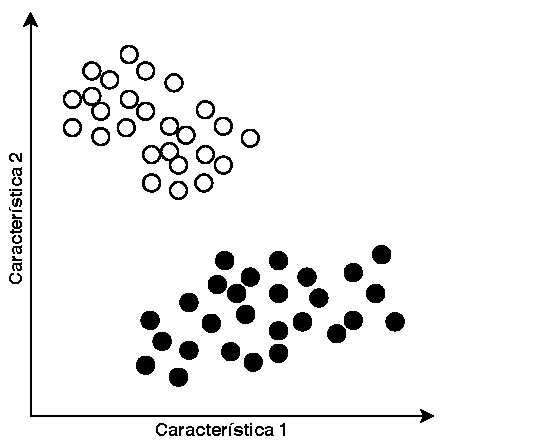
\includegraphics[scale=.80]{img/classificacao_a}}\qquad
  \subcaptionbox{\label{classificationB}}{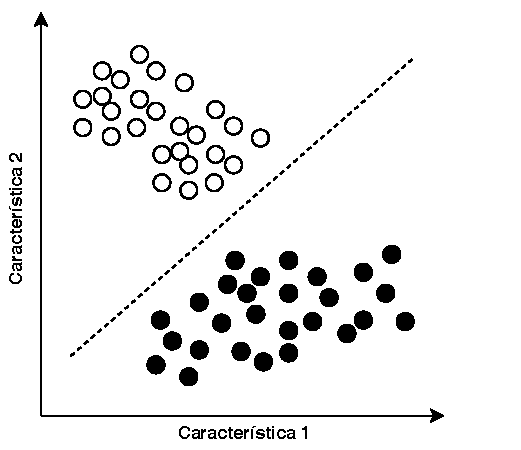
\includegraphics[scale=.80]{img/classificacao_b}}
  \vspace{1.5em}
  \Ididthis
\end{figure}

Em problemas de classificação, assumimos que são disponibilizados dados
etiquetados (classes) para gerar regras (i.e., gerar classificadores através do
treinamento) que podem ajudar a atribuir uma etiqueta a novos dados que não
possuem classes. Neste caso, podemos derivar uma regra exata pela
disponibilidade das classes. Na Figura \ref{classification} vemos uma ilustração
deste exemplo. É mostrado duas classes, etiquetadas com pontos brancos e pontos
pretos, e uma reta (Figura \ref{classificationB}) representado a regra que nos
ajuda a estabelecer uma classe para cada novo ponto
\cite{suthaharan2016machine}.

Uma técnica de classificação é uma abordagem sistemática para construção de
modelos de classificação a partir de dados de entrada. Cada técnica implementa
um algoritmo de aprendizagem para identificar um modelo que seja mais apropriado
para o relacionamento entre o conjunto de atributos e as classes dos dados
entrada. O modelo gerado pelo algoritmo de aprendizagem deve se adaptar aos
dados de entrada e prever corretamente os rótulos de classes de registros que
ele não teve contato antes. Ou seja, um dos principais objetivos do algoritmo de
aprendizagem é gerar modelos com grande capacidade de generalização
\cite{tan2009introduccao}.

\imagem{.7}{construcao_de_classificacao}{\label{classificationConstruction}
Abordagem geral para a construção de um modelo de classificação}
{\citeonline{tan2009introduccao}}

Em uma abordagem geral para a construção de um modelo de classificação,
primeiro, um conjunto de treinamento consistindo de registros com rótulos de
classe conhecido é fornecido. O conjunto de treinamento é usado para construir
um modelo de classificação, que é então aplicado a um conjunto de testes, i. e.
registros com rótulos desconhecidos para o modelo. A Figura
\ref{classificationConstruction} ilustra essa abordagem geral
\cite{tan2009introduccao}.

Segundo \citeonline{tan2009introduccao} a avaliação do desempenho de um modelo
de classificação é baseada na contagem de registros do conjunto de teste que
foram classificados correta e incorretamente. Estas contagens são organizadas em
uma tabela denominada matriz de confusão. O Quadro \ref{confusionMatrix}
apresenta uma matriz de confusão para um problema de classificação binária.
Baseado nas entradas da matriz de confusão, o número de previsões corretas
realizadas pelo modelo é \((f_{11} + f_{00})\) e o número de previsões
incorretas é \((f_{10} + f_{01})\).

\begin{quadro}[]
  \centering
  \caption{Exemplo de matriz de confusão}
  \label{confusionMatrix}
  \begin{tabular}{ll|c|c|}
    \cline{3-4}
    \multicolumn{1}{c}{\textbf{}} & \multicolumn{1}{c|}{\textbf{}} & \multicolumn{2}{l|}{\textbf{Classe prevista}} \\ \cline{3-4}
    & \multicolumn{1}{c|}{\textbf{}} & Classe = 1 & Classe = 0 \\ \hline
    \multicolumn{1}{|l|}{\multirow{2}{*}{\textbf{Classe real}}} & Classe = 1 & $f_{11}$ & $f_{10}$ \\ \cline{2-4}
    \multicolumn{1}{|l|}{} & Classe = 0 & $f_{01}$ & $f_{00}$ \\ \hline
  \end{tabular}
  \Ididthis
\end{quadro}

A matriz de confusão mostra informações importantes para determinar a
performance do modelo, no entanto, resumir estas informações em um único número
é mais conveniente quando queremos comparar o desempenho entre  diferentes
modelos. Isto pode ser feito usando uma métrica de desempenho como a precisão,
que é definida da seguinte maneira \cite{tan2009introduccao}:
\[
  \text{Precisão} =
  \frac
    {\text{Número de previsões corretas}}
    {\text{Número total de previsões}} =
  \frac
    {f_{11} + f_{00}}
    {f_{11} + f_{10} + f_{01} + f_{00}}
\]

\subsubsection{Árvore de decisão}

Em ML, existem dois tipos de árvores de decisão: árvores de regressão e árvores
de classificação. Uma árvore de decisão utiliza uma abordagem baseada em regras
para dividir o domínio dos dados em múltiplos espaços lineares e prever
respostas. Se as respostas previstas forem contínuas, então a árvore de decisão
é chamada de árvore de regressão, e se as previsões são discretas, ou seja,
pertencem a uma classe, então a árvore de decisão é chamada de árvore de
classificação \cite{suthaharan2016machine}.

Segundo \citeonline{suthaharan2016machine}, árvores de decisão são modelos de
aprendizado supervisionado que mapeiam o domínio dos dados hierarquicamente em
um conjunto de respostas. Dividindo o domínio dos dados (também chamado de nó)
recursivamente em dois subdomínios de forma que os subdomínios tenham um maior
ganho de informação que o nó que foi dividido. Já que o objetivo do aprendizado
supervisionado é a classificação dos dados, portanto,  o aumento do ganho de
informação influencia na eficiência da classificação nos subdomínios criados
pela divisão. Encontrar a divisão que traga o máximo de ganho de informação, ou
seja, eficiência na classificação é o objetivo do dos algoritmos de otimização
no aprendizado supervisionado baseado em árvores de decisão.

\citeonline{suthaharan2016machine} traz um exemplo de classificação usando
árvore de decisão. Suponha que temos um sistema que produz eventos (observações)
que podem pertencer a uma de duas classes, \(0\) ou \(1\) (e.g., chuva ou não
chuva, cara ou coroa), e estes eventos dependem apenas de uma variável.
Consequentemente, definimos o domínio como: \(D = \{e_1, e_2, \ldots, e_n\}\)
(assumimos que isto é um conjunto ordenado), e seus rótulos de classe
correspondentes \(L = {r_1, r_2, r_3, \ldots, r_n}\), onde \(r_i\) pertence
\(\{0, 1\}\), e \(i = 1 \ldots n\). A propagação dos rótulos das classes sobre o
domínio dos dados determina a facilidade na classificação. Representamos o ganho
de informação do domínio \(D\) em relação a \(L\) por \(I_i\) e dividimos o
conjunto ordenado na localização \(m\) para formar dois subdomínios \(D_1 =
\{e_1, e_2, \ldots, e_m\}\) e \(D_2 = \{e_{m+1}, e_{m+2}, \ldots, e_n\}\) com os
conjuntos de respostas correspondentes \(L_1 = \{r_1, r_2, \ldots, r_m\}\) e
\(L_2 = \{r_{m+1}, r_{m+2}, \ldots, r_n\}\). Se os respectivos ganhos de
informação são \(I_{i1}\) e \(I_{i2}\), então \(m\) será considerado a melhor
divisão se a  \(\text{média}(I_{i1}, I_{i2}) > I_i\). Não obstante, precisamos
de uma boa medida quantitativa para mensurar o ganho de informação obtido após a
divisão dos dados.

Vamos supor que \(p_0\) e \(p_1\) representem as probabilidades de que as
classes \(0\) e \(1\) possam ser extraídas do domínio \(D\), respectivamente.
Se, por exemplo, \(|p_0 - p_1| \to 1\); então podemos observar que uma classe em
particular tem grande predominância neste domínio, portanto, não é mais
necessário dividir os dados. Similarmente, se \(|p_0 - p_1| \to 0\), então as
classes tem predominância igual no domínio; logo, uma divisão é necessária.
Neste caso geramos dois subdomínios \(D_1\) e \(D_2\). Digamos que, \(q_0\) e
\(q_1\) são as probabilidades de que a classe \(0\) e a classe \(1\) sejam
derivadas do subdomínio \(D_1\), respectivamente. Se a divisão for eficiente,
\(q_0 > p_0\) ou \(q_1 > p_1\). Assumindo \(q_0 > p_0\), então \(q_0 = p_0 +
\epsilon\), onde \(\epsilon > 0\).
\[|q_0 - q_1| = |2q_0 - 1| = |2(p_0 + \epsilon) - 1| = |2p_0 + 2\epsilon - 1|\]
\[|q_0 - q_1| = |p_0 + 1 - p_1 + 2\epsilon - 1| = |p_0 - p_1 + 2\epsilon|\]
Esta equação enfatiza a seguinte inequação, (quando \(q_0 > p_0)\):
\[|q_0 - q_1| > |p_0 - p_1|\]

\imagem{.60}{decision_tree}{\label{decisionTree}Exemplo de árvore de decisão usada para classificação construída com um domínio de dados uni-dimensional}{\citeonline{suthaharan2016machine}}

As diferenças absolutas na inequação acima são as medidas quantitativas de
proporcionalidade entre as classes em seus respectivos subdomínios. Esta medida
probabilística é uma boa métrica para abordagem de otimização de árvores de
decisão. Na Figura \ref{decisionTree} vemos um exemplo de árvore de decisão em
termos de divisão de domínios focado no ganho de informação.

\subsubsection{K-ésimo vizinho mais próximo}

\apudonline{fix1951discriminatory}{peterson2009knn} introduziram um método não
paramétrico de reconhecimento de padrões que ficou conhecido como Regra do
K-ésimo Vizinho Mais Próximo (do inglês, \textit{K-nearest-neighbor}, KNN). O
KNN é um dos algoritmos de classificação mais simples e mais fundamentais e
deveria ser a primeira escolha para um estudo de classificação quando se tem
pouco ou nenhum conhecimento sobre a distribuição dos dados. A classificação com
KNN foi desenvolvida a partir da necessidade de realizar análises
discriminatórias quando estimativas confiáveis de densidade de probabilidade dos
dados não são conhecidas ou difíceis de determinar.
\apudonline{cover1967nearest}{peterson2009knn} descreveram as propriedades
formais do KNN, por exemplo, foi demonstrado que para \(k = 1\) e \(n \to
\infty\) o erro de classificação do KNN é limitado pelo dobro da taxa de erro de
Bayes. Desde que essas propriedades formais foram estabelecidas seguiu-se uma
longa linha de investigações incluindo uma abordagem de rejeição
\apud{hellman1970nearest}{peterson2009knn}, melhoramento em relação com a taxa
de erro de Bayes \apud{fukunaga1975k}{peterson2009knn}, abordagem com pesos nas
distâncias \apud{dudani1976distance}{peterson2009knn}.

\begin{figure}[!htb]
  \centering
  \caption{\label{knn} Os 1, 2 e 3 vizinhos mais próximos de um ponto dado}
  \subcaptionbox{\label{knnA}1-vizinho mais próximo}{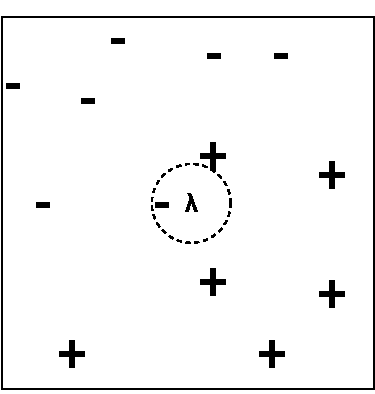
\includegraphics[scale=.75]{img/knn_example_a}}\qquad
  \subcaptionbox{\label{knnB}2-vizinhos mais próximo}{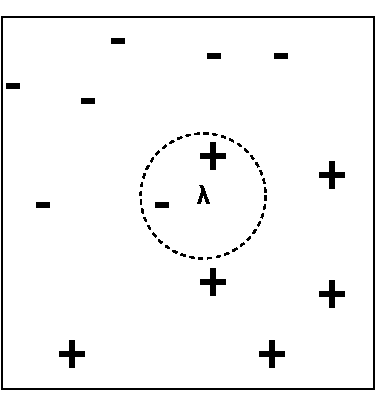
\includegraphics[scale=.75]{img/knn_example_b}}\qquad
  \subcaptionbox{\label{knnC}3-vizinhos mais próximo}{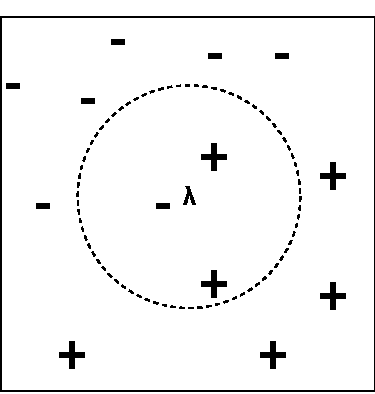
\includegraphics[scale=.75]{img/knn_example_c}}
  \vspace{1.5em}
  \Otherguydidthis{tan2009introduccao}
\end{figure}

Segundo \citeonline{tan2009introduccao} um classificador que utiliza KNN
representa cada exemplo, de treinamento ou de teste, como um ponto de dado em um
espaço \(d\)-dimensional, onde \(d\) é a quantidade de atributos. Dado um
exemplo de teste, calcula-se a sua proximidade com o resto dos pontos de dados
do conjunto de treinamento, usando alguma medida de distância, geralmente a
distância euclidiana. Os \(k\) vizinhos mais próximos de um determinado ponto de
teste \(z\) se referem aos \(k\) pontos com menor distância de \(z\). Então,
\(z\) é classificado com base nos rótulos de classe do seus vizinhos mais
próximos e lhe é atribuída a classe majoritária dos seus vizinhos mais próximos.
No exemplo da Figura \ref{knn} determinamos que o símbolo \(\textbf{-}\)
representa a classe negativo e o símbolo \(\textbf{+}\) representa a classe
positivo e \(\lambda\) representa um ponto dado a ser classificado. Na Figura
\ref{knnA}, onde \(k = 1\), foi atribuído ao ponto dado a classe negativo. Na
Figura \ref{knnB}, com \(k = 2\), os dois vizinhos mais próximos do ponto dado
tem classes distintas, portanto, podemos atribuir aleatoriamente qualquer uma
das duas classes. Na Figura \ref{knnC}, com \(k = 3\), dois dos vizinhos mais
próximos do ponto dado são da classe positivo e apenas um é da classe negativo,
logo, atribuímos ao ponto dado a classe positivo.

O desempenho de um classificador usando KNN pode ser melhorado quando os
atributos são transformados antes da análise de classificação. A forma mais
comum de transformação é a normalização ou padronização. A normalização remove
efeitos provocados por atributos com escalas diferentes, exemplo, o atributo
peso de um paciente pode ser baseado na unidade quilograma enquanto os valores
de proteína no sangue são baseados em nanograma por decilitro variando entre
\(-3\) e \(3\), logo, o peso do paciente teria maior influência no cálculo das
distâncias entre os pontos de exemplo e, por consequência, na classificação
\cite{peterson2009knn}.

\subsubsection{Regressão logística}

A Regressão Logística (RL) é uma generalização da regressão linear. É usada
principalmente para prever variáveis dependentes binárias ou de múltiplas
classes. Como a variável de resposta é discreta, ela não pode ser modelada
diretamente por regressão linear. Portanto, em vez de prever uma estimativa de
ponto do evento em si, o modelo baseia-se para prever a probabilidade de sua
ocorrência \cite{csen2012predicting}.

O modelos de RL surge do desejo de modelar as probabilidades posteriores de de
\(K\) classes através de funções lineares em \(x\), ao mesmo tempo, garantir que
a soma dessas probabilidades seja um e elas permaneçam no intervalo entre \(0\)
e \(1\) \cite{james2013introduction}.

\imagem{.5}{logistic_regression}{\label{logisticRegression}Previsões utilizando
regressão logística. As probabilidades se encontram no intervalo entre 0 e
1}{\citeonline{james2013introduction}}

Uma vantagem da RL no processo de classificação de uma variável dependente
binária (binomial), é que, nela, pode ser usado um conjunto de variáveis
independentes numéricas ou categóricas \cite{kleinbaum2002analysis}.

Dada uma variável ou conjunto de variáveis \(X\), podemos utilizar um modelo de
RL para calcular a probabilidade de pertencimento à classe \(y\). Para cada
valor ou valores de \(X\) pode ser feita uma previsão para a classe \(y\). Por
exemplo, pode-se dizer que o item sendo testado pertence a classe \(y\) sempre
que o modelo RL retornar uma probabilidade maior que 50\%, sendo que este limiar
pode ser ajustado de acordo com a necessidade do problema abordado
\cite{james2013introduction}.

Os modelos de RL para diversas variáveis é descrito pela seguinte fórmula:
\[\text{logit}(p_i)
= \text{ln}\left(\frac{p_i}{1 - p_i}\right)
= \beta_0 + \beta_1 X_{1,i} + \ldots + \beta_k X_{k,i}\]

Onde, \(\beta_0\), \(\beta_1\), \ldots, \(\beta_k\) são os coeficientes das
variáveis que explicam a ocorrência de determinado evento \(p_i\) é a
probabilidade de um evento ocorrer dado o conjunto de variáveis \(i\).

O resultado do modelo logit é uma curva em forma de S (Figura
\ref{logisticRegression}).  Para estimar um modelo de regressão logística, essa
curva de valores previstos é ajustada aos dados reais, analogamente como é feito
com uma relação linear em regressão múltipla.

Em níveis muito baixos da variável independente, a probabilidade se aproxima de
0\%, mas nunca alcança tal valor. Da mesma forma, quando o valor da variável
independente aumenta, os valores previstos crescem para acima da curva, mas, em
seguida, a inclinação começa a diminuir, aproximando a probabilidade de 100\%,
sem, entretanto, exceder esse valor \cite{hair2009analise}.

\section{Trabalhos relacionados}

\citeonline{ramos2018estudo}, analisaram a performance de diferentes algoritmos
na previsão da evasão em alunos EAD. Neste trabalho foram utilizados dados de
turmas de dois cursos de graduação na Universidade de Pernambuco (UPE). Os
algoritmos testados foram: Árvore de Decisão, Máquina de Vetor de Suporte
(SVM), Rede Neural Artificial, K-Vizinhos Mais Próximos (KNN) e Regressão
Logística. As variáveis foram construídas com base na TDT. O algoritmo com maior
acurácia foi o KNN, com maior precisão foi o SVM e a Regressão Logística teve os
maiores valores de Recall e Área Sob a Curva ROC (AUC).

\citeonline{queiroga2018modelo}, elaboraram um modelo de predição da evasão de
estudantes em cursos técnicos a distância, através de mineração de dados,
utilizando dados de turmas EAD do Câmpus Visconde da Graça (CaVG) do Instituto
Federal Sul-rio-grandense (IFSul). Os algoritmos utilizados para gerar os
modelos testados foram: \textit{Bayes Net}, \textit{Simple Logistic},
\textit{Multilayer Perceptron}, \textit{Random Forest} e J48, implementados na
biblioteca WEKA. Todos os algoritmos selecionados previram com exatidão de 95\%
a evasão de um aluno antes do final do primeiro ano. O algoritmo que mais se
destacou no quesito acurácia foi o Random Forest com 85\%.

\citeonline{manhaes2011previsao}, utilizaram mineração de dados para identificar
antecipadamente alunos com risco de evasão. Foram utilizados dados de cursos de
graduação da Universidade Federal do Rio de Janeiro (UFRJ). Os resultados
mostraram que utilizando as primeiras notas semestrais dos calouros é possível
identificar com precisão de 80\% a situação final do aluno no curso.

\citeonline{paz2017identificando}, Aplicaram KDD em dados coletados em uma IES,
e, através da tarefa de classificação, utilizando a técnica de árvores de
decisão, atingiram acurácia de 90\% na identificação de alunos evasores.

\citeonline{ramos2016abordagem} desenvolveu e testou modelos preditivos baseados
nos algoritmos Árvore de Decisão (TreeDecision), Máquina de Vetor de Suporte
(SVM), Rede Neural Artificial (NeuralNet), k-Nearest Neighbors (KNN) e Regressão
Logística (RegLog), usando com base as variáveis representativas dos construtos
da distância transacional, obtidas em trabalho anterior
\cite{ramos2016mapeamento}. Esse trabalho serviu como principal referência para
o desenvolvimento deste estudo, a fim de verificar a aplicabilidade do método em
um outro cenário educacional.